\exercise{Fold normal form revisited}{4}
Consider the normal from of the fold bifurcation, which we can write as 
\eqn{
\dot{x}=ax^2+bp
}
where $a$ and $b$ are normal form coefficients, $p$ is the control parameter, and $x$ is the dynamical variable. Find the steady states, determine their stability, and draw the bifurcation diagram. Are there actually different forms (e.g.~subcritical, supercritical) of this bifurcation as well?

\solution
We compute the steady states by solving 
\eq{
0=ax^2+bp
}
which yields 
\eq{
x^*=\pm \sqrt{\frac{b}{a}p}
}
This means we have either two steady states ($bp/a>0$) or none ($bp/a<0$). If $b/a>0$ we find the steady states at positive values of $p$, otherwise they only exist at negative values of $p$. 

In this sense there are two forms of the fold bifurcation, but they are indistinguishable in practice.

To determine the stability of solutions we compute
\eq{
f_{\rm x}=\frac{\partial }{\partial x} ax^2+bp = 2ax
}
If $a>0$ then the steady state at $+\sqrt{bp/a}$ is unstable and the one at $+\sqrt{bp/a}$ is stable. Otherwise its the other way around. 

We can now draw the bifurcation diagram 
\begin{center}
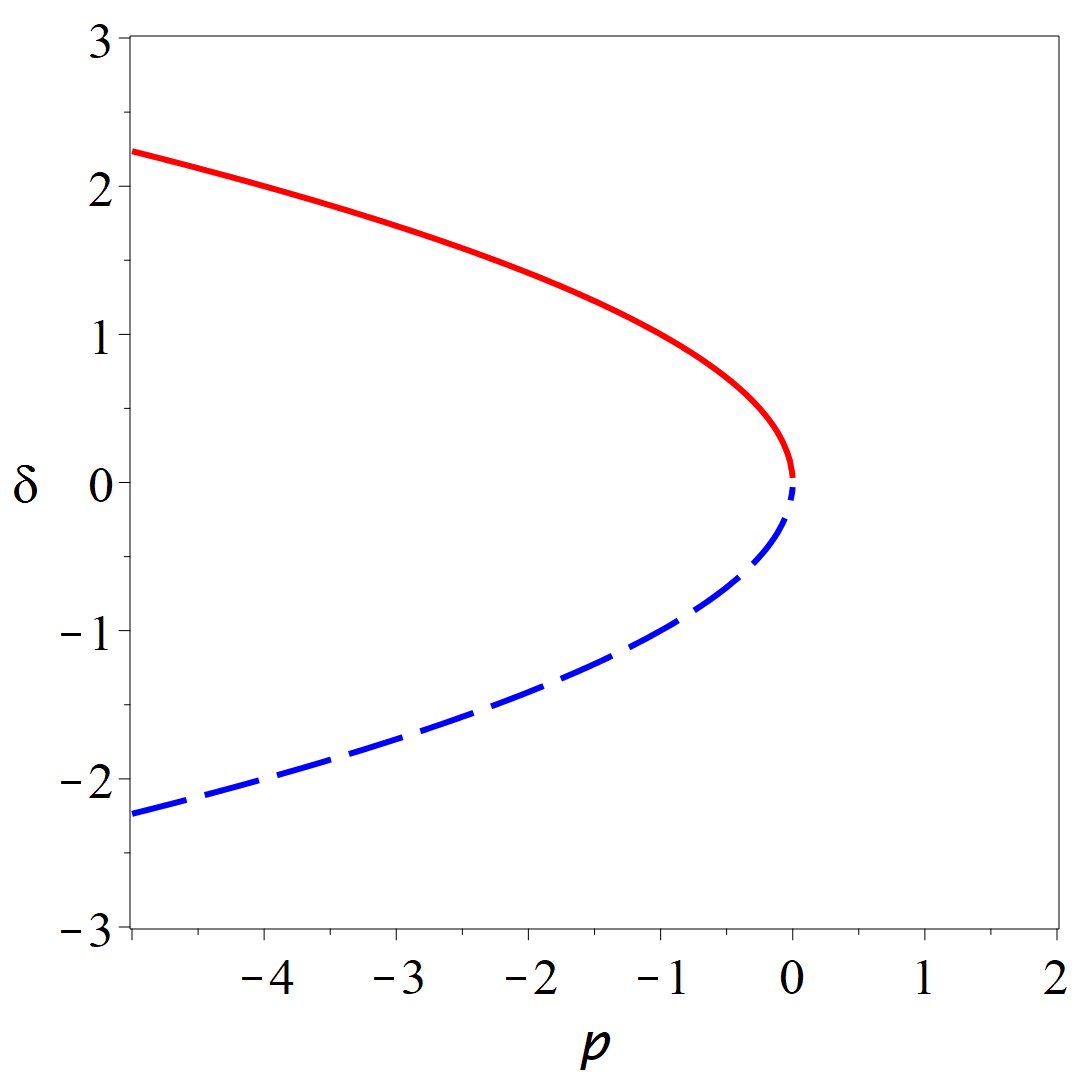
\includegraphics[width=0.6\textwidth]{Fold}
\end{center}
This diagram corresponds to the case $a<0$ (positive branch of steady states is stable) and $b>0$ (steady states exist for negative $p$).
